%%%%%%%%%%%%%%%%%%%%%%%%%%%%%%%%%%%%%%%%%
% Beamer Presentation
% LaTeX Template
% Version 2.0 (March 8, 2022)
%
% This template originates from:
% https://www.LaTeXTemplates.com
%
% Author:
% Vel (vel@latextemplates.com)
%
% License:
% CC BY-NC-SA 4.0 (https://creativecommons.org/licenses/by-nc-sa/4.0/)
%
%%%%%%%%%%%%%%%%%%%%%%%%%%%%%%%%%%%%%%%%%

%----------------------------------------------------------------------------------------
%	PACKAGES AND OTHER DOCUMENT CONFIGURATIONS
%----------------------------------------------------------------------------------------

\documentclass[
	10pt, % Set the default font size, options include: 8pt, 9pt, 10pt, 11pt, 12pt, 14pt, 17pt, 20pt
	t, % Uncomment to vertically align all slide content to the top of the slide, rather than the default centered
	%aspectratio=169, % Uncomment to set the aspect ratio to a 16:9 ratio which matches the aspect ratio of 1080p and 4K screens and projectors
]{beamer}

\graphicspath{{Images/}{./}} % Specifies where to look for included images (trailing slash required)

\usepackage{booktabs} % Allows the use of \toprule, \midrule and \bottomrule for better rules in tables
\usepackage{graphicx}
\usepackage{caption}
\usepackage{subcaption}
\usepackage{hyperref}
\usepackage[english,brazil]{babel}
\RequirePackage[backend=biber,
style=ieee,
%style=authoryear,
%style=authoryear-comp,
%style=authoryear-ibid,
%style=authoryear-icomp,
%style=authoryear-icomp,
citestyle=authoryear,
]{biblatex}

%----------------------------------------------------------------------------------------
%	SELECT LAYOUT THEME
%----------------------------------------------------------------------------------------

% Beamer comes with a number of default layout themes which change the colors and layouts of slides. Below is a list of all themes available, uncomment each in turn to see what they look like.

%\usetheme{default}
%\usetheme{AnnArbor}
%\usetheme{Antibes}
%\usetheme{Bergen}
%\usetheme{Berkeley}
%\usetheme{Berlin}
%\usetheme{Boadilla}
%\usetheme{CambridgeUS}
%\usetheme{Copenhagen}
%\usetheme{Darmstadt}
%\usetheme{Dresden}
%\usetheme{Frankfurt}
%\usetheme{Goettingen}
%\usetheme{Hannover}
%\usetheme{Ilmenau}
%\usetheme{JuanLesPins}
%\usetheme{Luebeck}
\usetheme{Madrid}
%\usetheme{Malmoe}
%\usetheme{Marburg}
%\usetheme{Montpellier}
%\usetheme{PaloAlto}
%\usetheme{Pittsburgh}
%\usetheme{Rochester}
%\usetheme{Singapore}
%\usetheme{Szeged}
%\usetheme{Warsaw}

%----------------------------------------------------------------------------------------
%	SELECT COLOR THEME
%----------------------------------------------------------------------------------------

% Beamer comes with a number of color themes that can be applied to any layout theme to change its colors. Uncomment each of these in turn to see how they change the colors of your selected layout theme.

%\usecolortheme{albatross}
%\usecolortheme{beaver}
%\usecolortheme{beetle}
% \usecolortheme{crane}
%\usecolortheme{dolphin}
%\usecolortheme{dove}
%\usecolortheme{fly}
%\usecolortheme{lily}
%\usecolortheme{monarca}
%\usecolortheme{seagull}
%\usecolortheme{seahorse}
%\usecolortheme{spruce}
%\usecolortheme{whale}
%\usecolortheme{wolverine}

%----------------------------------------------------------------------------------------
%	SELECT FONT THEME & FONTS
%----------------------------------------------------------------------------------------

% Beamer comes with several font themes to easily change the fonts used in various parts of the presentation. Review the comments beside each one to decide if you would like to use it. Note that additional options can be specified for several of these font themes, consult the beamer documentation for more information.

\usefonttheme{default} % Typeset using the default sans serif font
%\usefonttheme{serif} % Typeset using the default serif font (make sure a sans font isn't being set as the default font if you use this option!)
%\usefonttheme{structurebold} % Typeset important structure text (titles, headlines, footlines, sidebar, etc) in bold
%\usefonttheme{structureitalicserif} % Typeset important structure text (titles, headlines, footlines, sidebar, etc) in italic serif
%\usefonttheme{structuresmallcapsserif} % Typeset important structure text (titles, headlines, footlines, sidebar, etc) in small caps serif

%------------------------------------------------

%\usepackage{mathptmx} % Use the Times font for serif text
\usepackage{palatino} % Use the Palatino font for serif text

%\usepackage{helvet} % Use the Helvetica font for sans serif text
% \usepackage[default]{opensans} % Use the Open Sans font for sans serif text
%\usepackage[default]{FiraSans} % Use the Fira Sans font for sans serif text
\usepackage[default]{lato} % Use the Lato font for sans serif text

%----------------------------------------------------------------------------------------
%	SELECT INNER THEME
%----------------------------------------------------------------------------------------

% Inner themes change the styling of internal slide elements, for example: bullet points, blocks, bibliography entries, title pages, theorems, etc. Uncomment each theme in turn to see what changes it makes to your presentation.

%\useinnertheme{default}
% \useinnertheme{circles}
\useinnertheme{rectangles}
%\useinnertheme{rounded}
%\useinnertheme{inmargin}

%----------------------------------------------------------------------------------------
%	SELECT OUTER THEME
%----------------------------------------------------------------------------------------

% Outer themes change the overall layout of slides, such as: header and footer lines, sidebars and slide titles. Uncomment each theme in turn to see what changes it makes to your presentation.

%\useoutertheme{default}
%\useoutertheme{infolines}
%\useoutertheme{miniframes}
%\useoutertheme{smoothbars}
%\useoutertheme{sidebar}
%\useoutertheme{split}
%\useoutertheme{shadow}
%\useoutertheme{tree}
%\useoutertheme{smoothtree}

%\setbeamertemplate{footline} % Uncomment this line to remove the footer line in all slides
%\setbeamertemplate{footline}[page number] % Uncomment this line to replace the footer line in all slides with a simple slide count

%\setbeamertemplate{navigation symbols}{} % Uncomment this line to remove the navigation symbols from the bottom of all slides

% \bibliography{references} % Specifies the bibliography file to include publications
% \bibliographystyle{apalike} % Specifies the bibliography style
\addbibresource{references.bib}

%----------------------------------------------------------------------------------------
%	PRESENTATION INFORMATION
%----------------------------------------------------------------------------------------

\title[DesWebII]{Desenvolvimento Web II} % The short title in the optional parameter appears at the bottom of every slide, the full title in the main parameter is only on the title page
\subtitle{Aula 01 - Introdução} % Presentation subtitle, remove this command if a subtitle isn't required
\author[Fabricio Bizotto]{Prof. Fabricio Bizotto} % Presenter name(s), the optional parameter can contain a shortened version to appear on the bottom of every slide, while the main parameter will appear on the title slide
\institute[IFC]{Instituto Federal Catarinense \\ \smallskip \textit{fabricio.bizotto@ifc.edu.br}} % Your institution, the optional parameter can be used for the institution shorthand and will appear on the bottom of every slide after author names, while the required parameter is used on the title slide and can include your email address or additional information on separate lines
\date[\today]{Ciência da Computação \\ \today} % Presentation date or conference/meeting name, the optional parameter can contain a shortened version to appear on the bottom of every slide, while the required parameter value is output to the title slide

%----------------------------------------------------------------------------------------
\begin{document}

%----------------------------------------------------------------------------------------
%	TITLE SLIDE
%----------------------------------------------------------------------------------------

\begin{frame}
	\titlepage % Output the title slide, automatically created using the text entered in the PRESENTATION INFORMATION block above
\end{frame}

%----------------------------------------------------------------------------------------
%	TABLE OF CONTENTS SLIDE
%----------------------------------------------------------------------------------------
% **Unidade 1: Introdução à Arquitetura de Sistemas Web (4 horas)**\
% 1.1. Conceitos básicos de arquitetura de sistemas web\
% 1.2. Modelos arquiteturais: monolítico, cliente-servidor, arquitetura em camadas, arquitetura orientada a serviços (SOA), arquitetura orientada a microsserviços\
% 1.3. Principais desafios e tendências\
% The table of contents outputs the sections and subsections that appear in your presentation, specified with the standard \section and \subsection commands. You may either display all sections and subsections on one slide with \tableofcontents, or display each section at a time on subsequent slides with \tableofcontents[pausesections]. The latter is useful if you want to step through each section and mention what you will discuss.

\begin{frame}
	\frametitle{Roteiro} % Slide title, remove this command for no title
	
	\tableofcontents % Output the table of contents (all sections on one slide)
	%\tableofcontents[pausesections] % Output the table of contents (break sections up across separate slides)
\end{frame}

%----------------------------------------------------------------------------------------
%	PRESENTATION BODY SLIDES
%----------------------------------------------------------------------------------------

\section{Introdução a Arquitetura de Software} % Sections are added in order to organize your presentation into discrete blocks, all sections and subsections are automatically output to the table of contents as an overview of the talk but NOT output in the presentation as separate slides

%------------------------------------------------

\subsection{Conceitos}

\begin{frame}
	\frametitle{Conceitos}
	
	A \alert{arquitetura da aplicação} descreve a estrutura interna e interações entre seus componentes. A arquitetura de uma aplicação é composta por:

	\begin{itemize}
		\item \textbf{Componentes}: partes que compõem a aplicação. Exemplos: cliente, servidor, banco de dados, etc.
		\item \textbf{Conectores}: mecanismos que permitem a comunicação entre os componentes. Exemplos: protocolos de comunicação, APIs, etc.
		\item \textbf{Restrições}: regras que definem como os componentes e conectores podem interagir. Exemplos: autenticação, autorização, etc.
	\end{itemize}
	\bigskip % Vertical whitespace

	\begin{alertblock}{Tomada de Decisão}
		Escolher a arquitetura correta para uma aplicação é uma das decisões mais importantes que um arquiteto de software deve tomar.
	\end{alertblock}
\end{frame}

%------------------------------------------------

\subsection{Modelos Arquiteturais}
\subsubsection{Monolito}

\begin{frame}
	\begin{center}
		
		\bigskip\bigskip\bigskip\bigskip % Vertical whitespace
		{\Large Modelos Arquiteturais}
		
		\bigskip\bigskip % Vertical whitespace
		{\Huge Monolito}
		
		\smallskip
		{\small \textit{Monolithic}}
	\end{center}

\end{frame}

\begin{frame}
	\frametitle{Principais Arquiteturas de Software}
	\framesubtitle{Monolito - Definição}
	
	Abordagem tradicional no desenvolvimento de software na qual todos os componentes de uma aplicação são combinados em uma única unidade totalmente integrada. A aplicação é implantada como uma \alert{única base de código} que contém todas as funcionalidades.

\end{frame}

\begin{frame}
	\frametitle{Principais Arquiteturas de Software}
	\framesubtitle{Monolito - Vantagens}

	\begin{exampleblock}{Vantagens}
		\begin{itemize}
			\item \textbf{Simplicidade da Arquitetura}: não existem muitas camadas e componentes para gerenciar. É mais fácil para começar.
			\item \textbf{Tecnologias}: usar uma única linguagem de programação e tecnologias para desenvolver a aplicação pode facilitar o entendimento da equipe.
			\item \textbf{Fluxo de implantação}: o `deploy` é simples de fazer e gerenciar. Não há necessidade de implantar vários componentes separadamente.
		\end{itemize}
	\end{exampleblock}

\end{frame}

\begin{frame}
	\frametitle{Principais Arquiteturas de Software}
	\framesubtitle{Monolito - Desvantabens}

	\begin{alertblock}{Desvantagens}
		\begin{itemize}
			\item \textbf{Acoplamento forte}: a aplicação é uma única unidade totalmente integrada, o que significa que qualquer alteração em um componente pode afetar outros componentes da aplicação.
			\item \textbf{Escalabilidade limitada}:a aplicação é implantada como uma única unidade, o que significa que todos os componentes da aplicação devem ser escalados juntos horizontalmente.
			\item \textbf{Implantação única}: a aplicação é implantada como uma única unidade, o que significa que todos os componentes da aplicação devem ser implantados juntos. Qualquer alteração, por menor que seja, requer a implantação de toda a aplicação.
			\item \textbf{Tecnologias limitadas}: todos os componentes da aplicação devem ser desenvolvidos usando a mesma linguagem de programação e tecnologias.
		\end{itemize}
	\end{alertblock}

\end{frame}

\begin{frame}
	\frametitle{Principais Arquiteturas de Software}
	\framesubtitle{Monolito - Representação}
	
	\begin{figure}
		\centering
		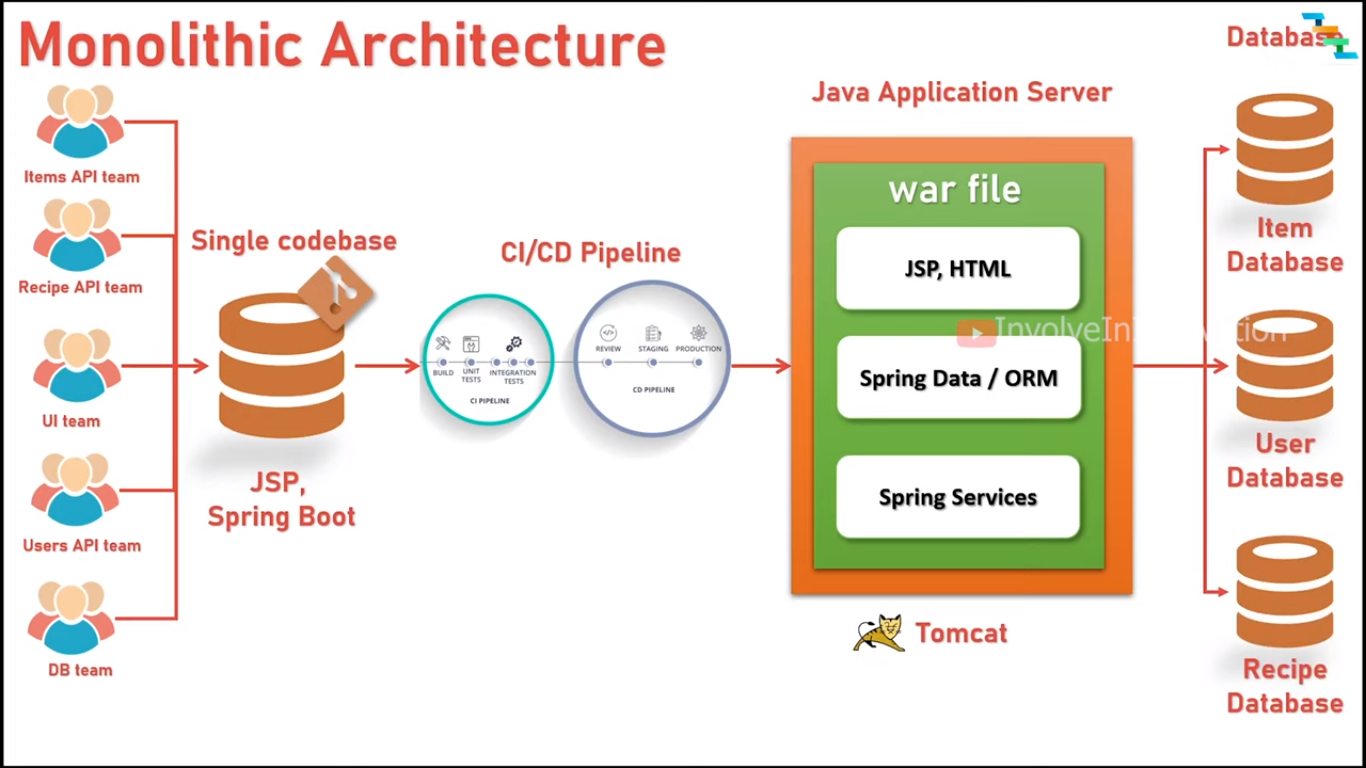
\includegraphics[width=0.9\linewidth]{Images/monolito2.png}
		\caption{Arquitetura Monolítica.}\label{fig:monolito}
	\end{figure}

\end{frame}

\begin{frame}
	\frametitle{Principais Arquiteturas de Software}
	\framesubtitle{Monolito - Escalando Horizontalmente}

	\begin{itemize}
		\item \textbf{Escalabilidade horizontal}: adicionar mais instâncias de um componente.
		\item \textbf{Escalabilidade vertical}: adicionar mais recursos (CPU, memória, etc) a um componente.
	\end{itemize}
	
	\begin{figure}
		\centering
		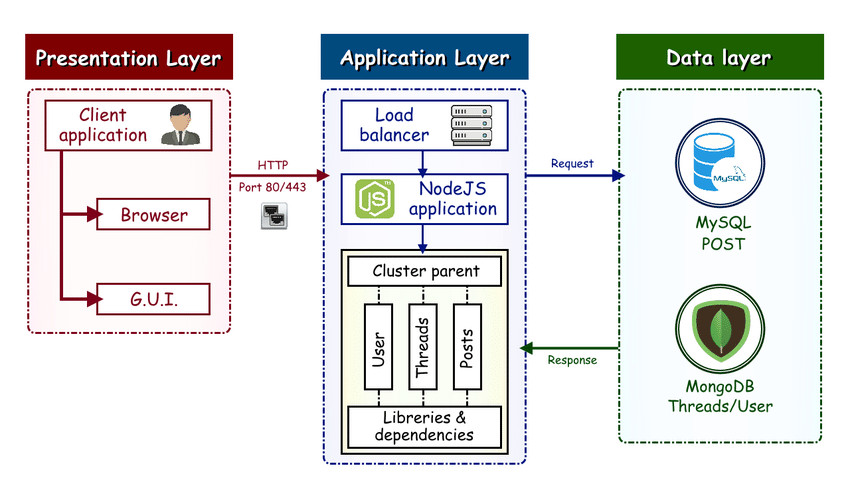
\includegraphics[width=0.8\linewidth]{Images/monolito-balancer.jpg}
		\caption{Arquitetura Monolítica com \textit{Load Balancer}.}\label{fig:monolito-balancer}
	\end{figure}

\end{frame}

\subsubsection{Arquitetura em N camadas (N-tier)}

\begin{frame}
	\begin{center}
		
		\bigskip\bigskip\bigskip\bigskip % Vertical whitespace
		{\Large Modelos Arquiteturais}
		
		\bigskip\bigskip % Vertical whitespace
		{\Huge N camadas}

		\smallskip
		{\small \textit{N-tier}}
	\end{center}

\end{frame}

\begin{frame}
	\frametitle{Principais Arquiteturas de Software}
	\framesubtitle{Arquitetura em N camadas (N-tier) - Definição}

	A arquitetura em N camadas é um padrão de arquitetura de software no qual a aplicação é dividida em camadas lógicas ou físicas.

	\begin{figure}
		\centering
		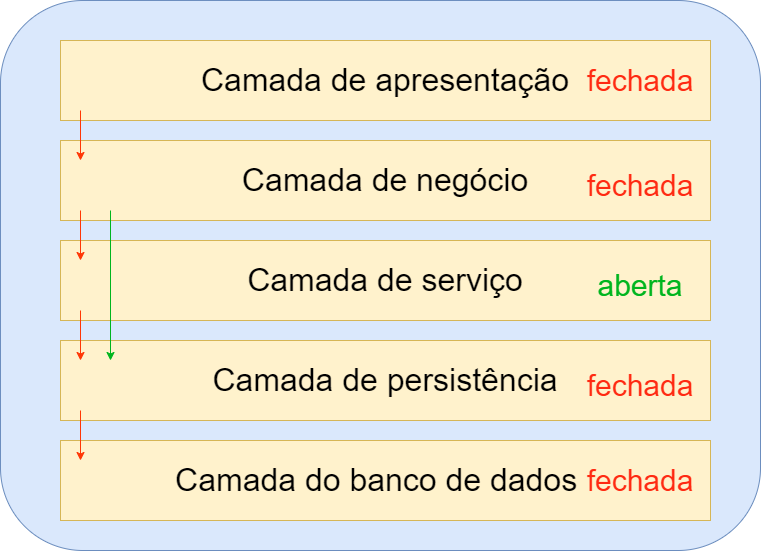
\includegraphics[width=0.6\linewidth]{Images/n-tier-simple-2.png}
		\caption{Arquitetura em camadas - Fluxo.}\label{fig:n-tier-simple-2}
	\end{figure}

\end{frame}

\begin{frame}
	\frametitle{Principais Arquiteturas de Software}
	\framesubtitle{Arquitetura em N camadas (N-tier) - Vantagens}

	\begin{exampleblock}{Vantagens}
		\begin{itemize}
			\item \textbf{Separação de Responsabilidades}: A separação clara das responsabilidades em diferentes camadas (como apresentação, lógica de negócios e acesso a dados) facilita a manutenção e a evolução do sistema.
			\item \textbf{Escalabilidade}: A escalabilidade é facilitada, pois cada camada pode ser dimensionada independentemente das outras, permitindo a otimização de recursos.
			\item \textbf{Facilidade de Testes}: Cada camada pode ser testada separadamente, o que simplifica os testes unitários e facilita a identificação e correção de falhas.
			\item \textbf{Manutenção}: Alterações em uma camada específica não devem afetar as outras, tornando a manutenção mais simples e menos propensa a efeitos colaterais indesejados.
		\end{itemize}
	\end{exampleblock}

\end{frame}

\begin{frame}
	\frametitle{Principais Arquiteturas de Software}
	\framesubtitle{Arquitetura em N camadas (N-tier) - Desvantagens}

	\begin{alertblock}{Desvantagens}
		\begin{itemize}
			\item \textbf{Complexidade Inicial}: A implementação de uma arquitetura em camadas pode ser mais complexa inicialmente, especialmente para projetos pequenos ou simples.
			\item \textbf{Comunicação entre camadas}: A comunicação entre camadas pode resultar em algum overhead, especialmente em sistemas distribuídos, o que pode impactar o desempenho. Alguns exemplos são latência, serialização e desserialização de dados, etc.
			\item \textbf{Duplicação de Lógica}: Pode ocorrer uma duplicação de lógica entre as camadas, o que pode levar a inconsistências se não for gerenciado adequadamente.
		\end{itemize}
	\end{alertblock}

\end{frame}

\begin{frame}
	\frametitle{Principais Arquiteturas de Software}
	\framesubtitle{Arquitetura em N camadas (N-tier) - Representação}
	
	\begin{figure}
		\centering
		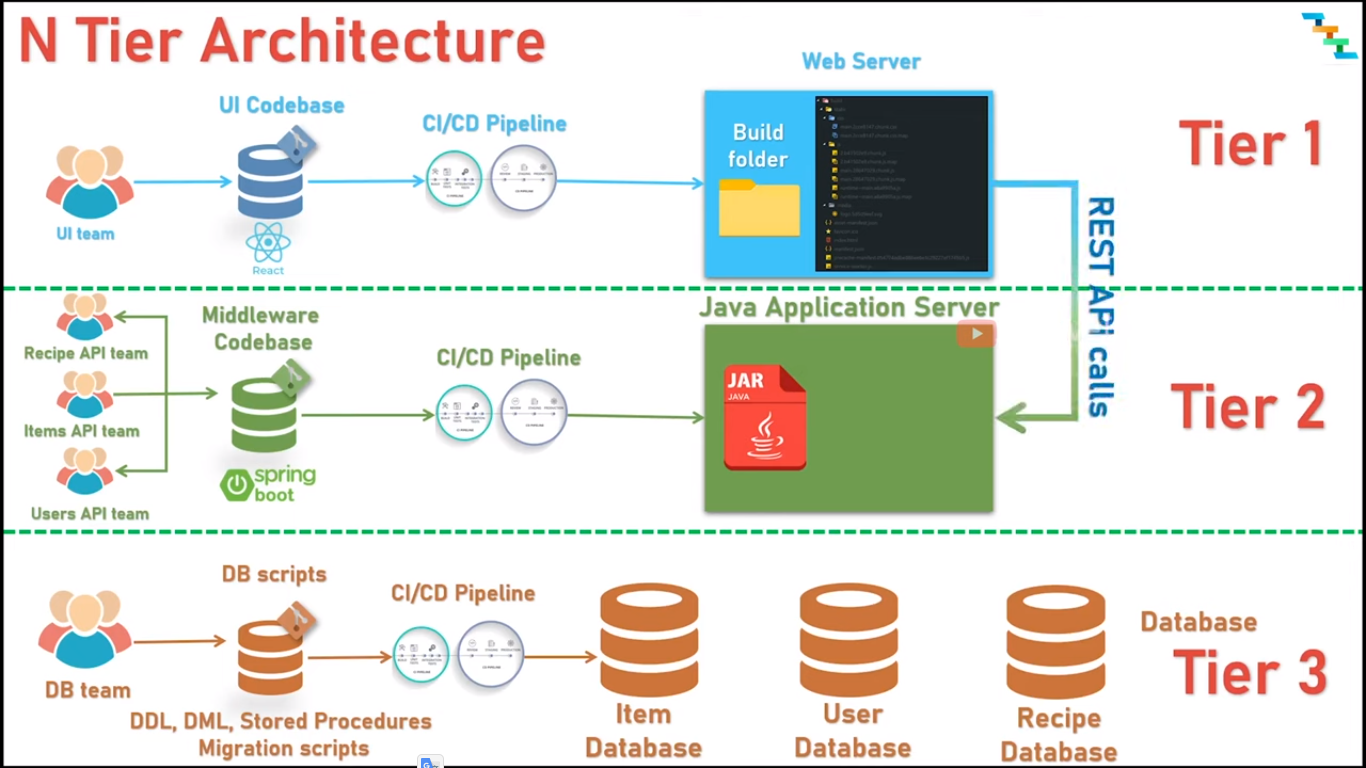
\includegraphics[width=0.9\linewidth]{Images/n-tier.png}
		\caption{Arquitetura em N camadas (N-tier).}\label{fig:n-tier}
	\end{figure}

\end{frame}

\begin{frame}
	\frametitle{Principais Arquiteturas de Software}
	\framesubtitle{Arquitetura em 2 camadas - Cliente-Servidor}

	A arquitetura de software em duas camadas, também conhecida como arquitetura cliente-servidor, é um modelo simples no qual a lógica de aplicação é dividida em duas partes principais: a camada de apresentação (cliente) e a camada de dados (servidor). Essa arquitetura é bastante direta e é frequentemente utilizada em aplicações pequenas e simples.
	
	\begin{figure}
		\centering
		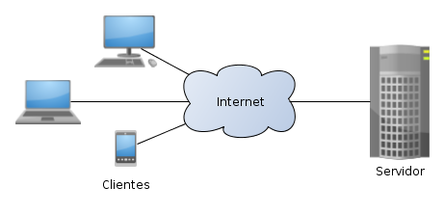
\includegraphics[width=0.7\linewidth]{Images/cliente-servidor.png}
		\caption{Arquitetura Cliente-Servidor.}\label{fig:cliente-servidor}
	\end{figure}

\end{frame}

\subsubsection{Microserviços}

\begin{frame}
	\begin{center}
		
		\bigskip\bigskip\bigskip\bigskip % Vertical whitespace
		{\Large Modelos Arquiteturais}
		
		\bigskip\bigskip % Vertical whitespace
		{\Huge Microserviços}
		
		\smallskip
		{\small \textit{Microservices}}
	\end{center}

\end{frame}

\begin{frame}
	\frametitle{Principais Arquiteturas de Software}
	\framesubtitle{Microserviços - Definição}

	\begin{itemize}
		\item A arquitetura de microsserviços é uma abordagem arquitetônica e organizacional do desenvolvimento de software na qual o software consiste em \alert{pequenos serviços independentes}.
		\item É similar à \alert{arquitetura orientada a serviços (SOA)}, mas com algumas diferenças importantes, tais como, por exemplo, o tamanho dos serviços e a forma como eles se comunicam.
		\item Esses serviços são mantidos por \alert{pequenas equipes autossuficientes}.
		\item Cada serviço é desenvolvido, implantado e gerenciado de forma \alert{independente}.
		\item Cada serviço é responsável por uma \alert{única funcionalidade}.
		\item Os serviços se comunicam entre si através de \alert{APIs} bem definidas.
	\end{itemize}

\end{frame}

\begin{frame}
	\frametitle{Principais Arquiteturas de Software}
	\framesubtitle{Microserviços - Vantagens}

	\begin{exampleblock}{Vantagens}
		\begin{itemize}
			\item \textbf{Separação de Responsabilidades}: Tudo é desenvolvido através de pequenas unidades de código e publicado em processos de deploy automatizados e independentes.
			\item \textbf{Tecnologias}: Essa abordagem permite que cada serviço seja desenvolvido usando a \textit{stack} mais adequadas para o problema que está sendo resolvido.
			\item \textbf{Aplicabilidade}: em aplicações de \alert{grande porte e complexas} que precisam ser escaladas rapidamente e com equipes distribuídas.
		\end{itemize}
	\end{exampleblock}
\end{frame}

\begin{frame}
	\frametitle{Principais Arquiteturas de Software}
	\framesubtitle{Microserviços - Desvantagens}

	\begin{alertblock}{Desvantagens}
		\begin{itemize}
			\item \textbf{Complexidade}: A complexidade de uma arquitetura de microsserviços é maior do que a de uma arquitetura monolítica, pois existem mais componentes para gerenciar.
			\item \textbf{Comunicação}: A comunicação entre os serviços pode resultar em algum overhead, especialmente em sistemas distribuídos, o que pode impactar o desempenho.
			\item \textbf{Testes}: Os testes de integração são mais complexos, pois envolvem a comunicação entre os serviços.
			\item \textbf{Gerenciamento}: O gerenciamento de uma arquitetura de microsserviços (governança) é mais complexo, pois existem mais componentes para gerenciar.
		\end{itemize}
	\end{alertblock}

\end{frame}

\begin{frame}
	\frametitle{Principais Arquiteturas de Software}
	\framesubtitle{Microserviços - Representação}
	
	\begin{figure}
		\centering
		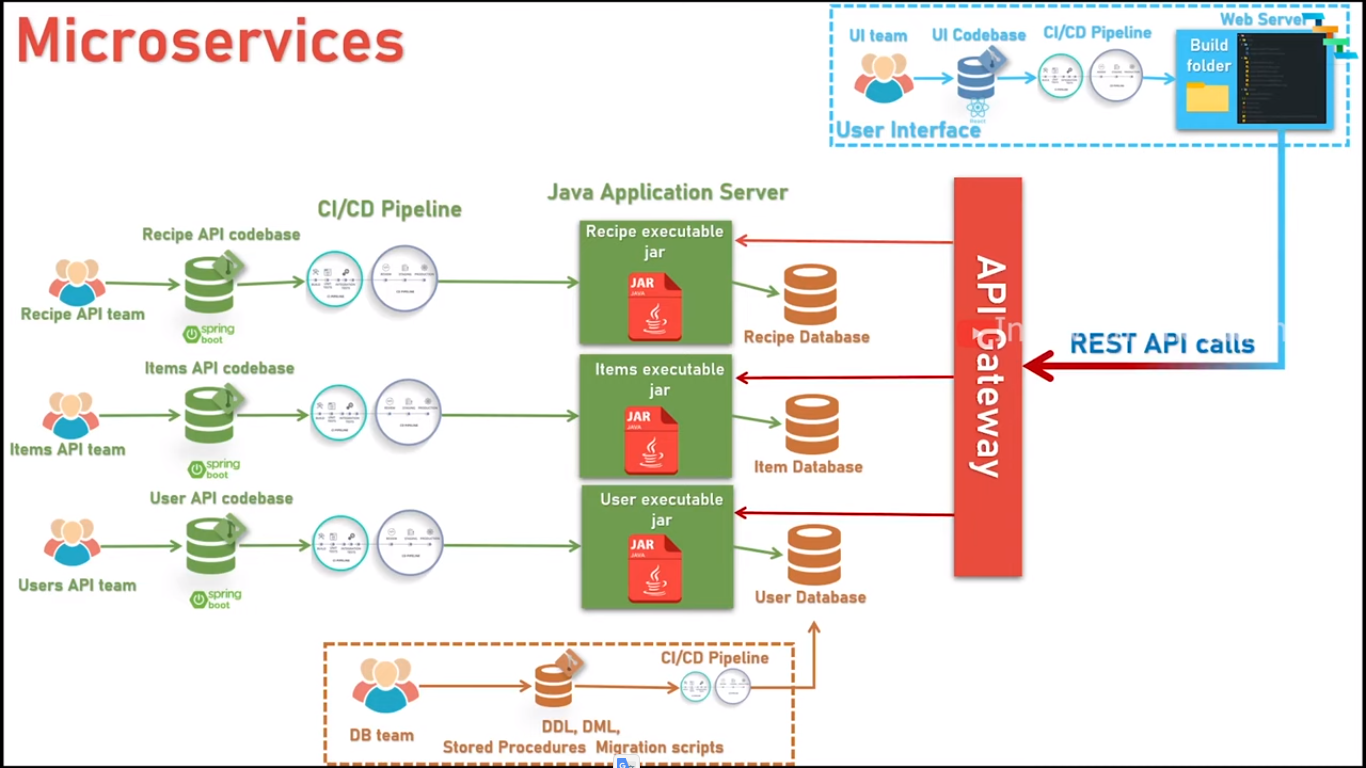
\includegraphics[width=0.9\linewidth]{Images/microservice.png}
		\caption{Arquitetura de Microsserviços.}\label{fig:microservices}
	\end{figure}

\end{frame}

\subsection{Comparativos}

\begin{frame}
	\begin{center}
		
		\bigskip\bigskip\bigskip\bigskip % Vertical whitespace
		{\Large Modelos Arquiteturais}
		
		\bigskip\bigskip % Vertical whitespace
		{\Huge Comparativos}
		
		% \smallskip
		% {\small \textit{Monolithic}}
	\end{center}

\end{frame}

\begin{frame}
	\frametitle{Principais Arquiteturas de Software}
	\framesubtitle{Monolito vs. Microsserviços}

	\begin{figure}
		\centering
		% \caption*{Fonte: \url{https://aws.amazon.com/pt/microservices/}}
		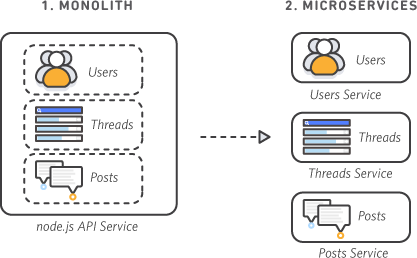
\includegraphics[width=0.9\linewidth]{Images/mono_x_micro.png}
		\caption{Monolito vs. Microsserviços.}\label{fig:monolito-vs-microservicos}
	\end{figure}

\end{frame}

\begin{frame}
	\frametitle{Principais Arquiteturas de Software}
	\framesubtitle{Monolito, N Camares e Microsserviços}

	\begin{figure}
		\centering
		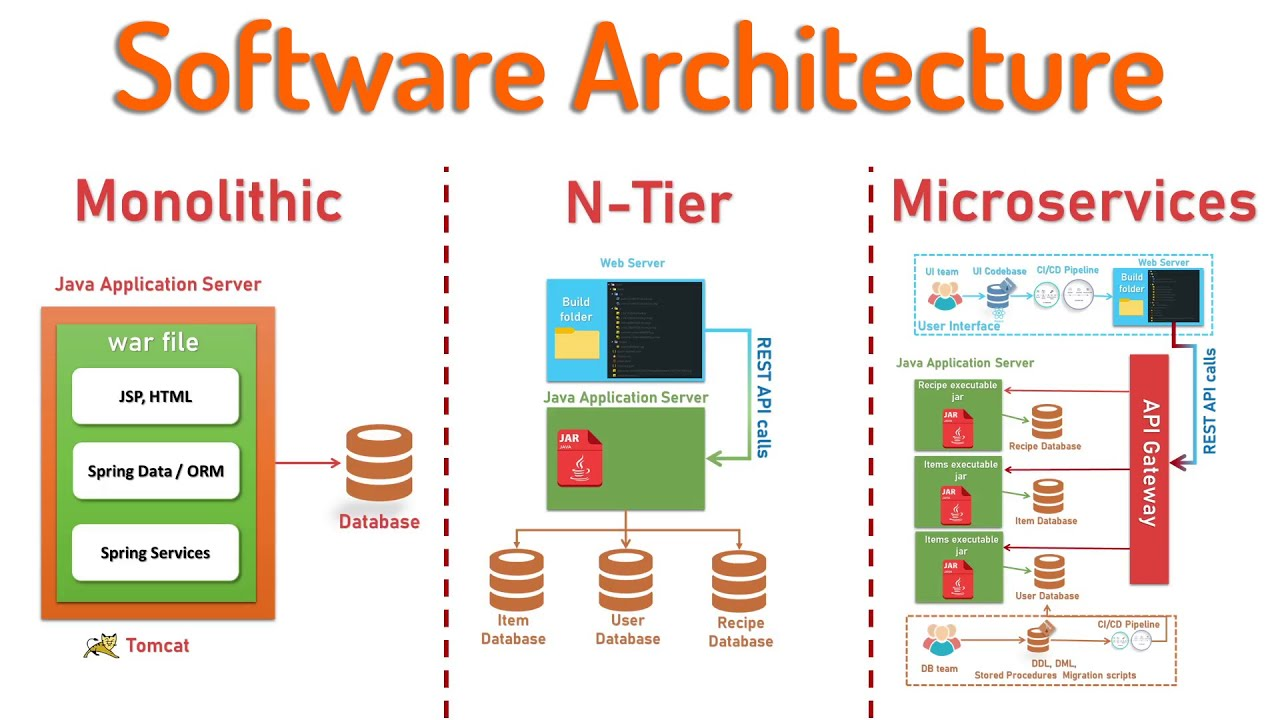
\includegraphics[width=0.9\linewidth]{Images/arquit-comparativo.jpg}
		\caption{Monolito, N Camares e Microsserviços.}\label{fig:comparativo}
	\end{figure}

\end{frame}

\begin{frame}
	\frametitle{Principais Arquiteturas de Software}
	\framesubtitle{Exemplo Prático}

	\textbf{Sistema de Comércio Eletrônico - Módulo de Recomendações:}

	\begin{exampleblock}{Monolito - Exemplo}
		Um componente que fornece recomendações de produtos com base no histórico de compras, comportamentos de navegação e preferências do usuário. Todos os módulos serão construídos na mesma base de código e implantados como uma única unidade.
	\end{exampleblock}

	\begin{exampleblock}{N Camadas - Exemplo}
		Será organizado como parte da camada de lógica de negócios (Backend).
	\end{exampleblock}

	\begin{exampleblock}{Microserviços - Exemplo}
		Um microserviço que fornece recomendações personalizadas aos clientes com base em seu histórico de compras, preferências e comportamentos de navegação. Será um serviço separado e independente.
	\end{exampleblock}
	

\end{frame}

\section{Outras Arquiteturas}

\begin{frame}
	\begin{center}
		
		\bigskip\bigskip\bigskip\bigskip % Vertical whitespace
		{\Large Modelos Arquiteturais}
		
		\bigskip\bigskip % Vertical whitespace
		{\Huge Outras Arquiteturas}
		
		% \smallskip
		% {\small \textit{Monolithic}}
	\end{center}

\end{frame}


\begin{frame}
	\frametitle{Outras Arquiteturas}
	\framesubtitle{Arquitetura Orientada a Serviços (SOA)}

	\begin{block}{Arquitetura Orientada a Serviços (SOA)}
		A arquitetura de microsserviços é uma evolução do estilo de arquitetura SOA. Embora cada serviço de SOA seja um \alert{recurso de negócios completo}, cada microsserviço é um componente de software muito menor, especializado em apenas uma única tarefa. Os microsserviços abordam as deficiências da SOA para tornar o software mais compatível com ambientes corporativos modernos baseados na nuvem \parencite{AWSSOA2024}.		
	\end{block}
	\begin{exampleblock}{Exemplo}
		\textbf{Sistema de Comércio Eletrônico - Serviço de Pagamento:} Responsável pelo processamento de transações financeiras, integração com gateways de pagamento e validação de transações.
	\end{exampleblock}
	
\end{frame}

\begin{frame}
	\frametitle{Outras Arquiteturas}
	\framesubtitle{Arquitetura Orientada a Eventos}

	\begin{block}{Arquitetura Orientada a Eventos}
		Uma arquitetura orientada por eventos usa eventos para acionamento e comunicação entre serviços desacoplados e é comum em aplicações modernas criadas com microsserviços \parencite{AWSEVENTOS2024}.
	\end{block}

	\begin{exampleblock}{Exemplo}
		\textbf{Sistema de Comércio Eletrônico - Pedido Realizado}: quando um cliente faz um pedido, um evento é gerado e enviado para o serviço de processamento de pedidos, que pode então iniciar o processamento do pedido.
	\end{exampleblock}
	
\end{frame}

\begin{frame}
	\frametitle{Outras Arquiteturas}
	\framesubtitle{Arquitetura Serverless}

	\begin{block}{Serverless}
		É um modelo de desenvolvimento nativo em nuvem para criação e execução de aplicações sem o gerenciamento de servidores. Os servidores ainda são usados nesse modelo, mas eles são abstraídos do desenvolvimento de aplicações \parencite{REDHAT2024}.
	\end{block}

	\begin{exampleblock}{Exemplo}
		\textbf{Serviço de Armazenamento (Storage)}: Os usuários fazem upload de imagens para um serviço de armazenamento na nuvem, como o Amazon S3. A função serverless terá a lógica para processar a imagem e gerar thumbnails em diferentes tamanhos.
	\end{exampleblock}
	
\end{frame}

%------------------------------------------------


\subsection{Material Complementar}

\begin{frame}
	\frametitle{Material Complementar}
	\framesubtitle{Vídeos, Podcasts, Livros, etc}
	
	\begin{itemize}
		\item \href{https://youtu.be/CsrHHHPHKwE}{\textbf{Aplicação Monolítica // Dicionário do Programador}}.\\Canal \textbf{Código Fonte TV}.
		\item \href{https://youtu.be/suZfVAk7hco}{\textbf{Arquitetura de Software: Monolítica x SOA x Microserviços}}.\\Canal \textbf{Marcos Dósea}.
		\item \href{https://www.youtube.com/watch?v=_2bDOCTnbKc}{\textbf{Microservices // Dicionário do Programador}}.\\Canal \textbf{Código Fonte TV}.
		\item \href{https://youtu.be/gtv9szE_P1U}{\textbf{Microservices na prática}}.\\Canal \textbf{Full Cycle}.
		\item \href{https://www.hipsters.tech/uma-linguagem-para-cada-combate-hipsters-ponto-tech-277}{\textbf{Microservices na prática}}.\\Podcast Hipsters Ponto Tech \textbf{Monolitos}.
	\end{itemize}
	
\end{frame}

\subsection{Quiz}

\begin{frame}
	\frametitle{Recapitulando}
	\framesubtitle{QUIZ}

	\vfill
	\begin{block}{Vamos praticar um pouco o que vimos até agora?}
		\href{https://quizizz.com/admin/quiz/65832b860b273f1989868234?source=quiz_share}{\textbf{QUIZ - Desenvolvimento Web - Arquitetura de Software}}
	\end{block}
	\vfill
		
\end{frame}

	
	
% \subsection{Modelos Arquiteturais para Web}

% \begin{frame}
% 	\begin{center}
		
% 		\bigskip\bigskip\bigskip\bigskip % Vertical whitespace
% 		{\Large Modelos Arquiteturais para Web}
		
% 		\bigskip\bigskip % Vertical whitespace
% 		{\Huge Modelo Cliente-Servidor}

% 		\begin{alertblock}{Observação}
% 			Não é uma arq
% 		\end{alertblock}
% 	\end{center}

% \end{frame}

%------------------------------------------------

% \subsection{Columns}

% \begin{frame}
% 	\frametitle{Multiple Columns}
% 	\framesubtitle{Subtitle} % Optional subtitle
	
% 	\begin{columns}[c] % The "c" option specifies centered vertical alignment while the "t" option is used for top vertical alignment
% 		\begin{column}{0.45\textwidth} % Left column width
% 			\textbf{Heading}
% 			\begin{enumerate}
% 				\item Statement
% 				\item Explanation
% 				\item Example
% 			\end{enumerate}
% 		\end{column}
% 		\begin{column}{0.5\textwidth} % Right column width
% 			Lorem ipsum dolor sit amet, consectetur adipiscing elit. Integer lectus nisl, ultricies in feugiat rutrum, porttitor sit amet augue. Aliquam ut tortor mauris. Sed volutpat ante purus, quis accumsan dolor.
% 		\end{column}
% 	\end{columns}
% \end{frame}

% %------------------------------------------------

% \section{Table and Figure Examples}

% \subsection{Table}

% \begin{frame}
% 	\frametitle{Table}
% 	\framesubtitle{Subtitle} % Optional subtitle
	
% 	\begin{table}
% 		\begin{tabular}{l l l}
% 			\toprule
% 			\textbf{Treatments} & \textbf{Response 1} & \textbf{Response 2}\\
% 			\midrule
% 			Treatment 1 & 0.0003262 & 0.562 \\
% 			Treatment 2 & 0.0015681 & 0.910 \\
% 			Treatment 3 & 0.0009271 & 0.296 \\
% 			\bottomrule
% 		\end{tabular}
% 		\caption{Table caption}
% 	\end{table}
% \end{frame}

% %------------------------------------------------

% \subsection{Figure}

% \begin{frame}
% 	\frametitle{Figure}
	
% 	\begin{figure}
% 		
\includegraphics[width=0.8\linewidth]{logo.png}
% 		\caption{IFC Videira.}
% 	\end{figure}
% \end{frame}

% %------------------------------------------------

% \section{Mathematics}

% \begin{frame}
% 	\frametitle{Definitions \& Examples}
	
% 	\begin{definition}
% 		A \alert{prime number} is a number that has exactly two divisors.
% 	\end{definition}
	
% 	\smallskip % Vertical whitespace
	
% 	\begin{example}
% 		\begin{itemize}
% 			\item 2 is prime (two divisors: 1 and 2).
% 			\item 3 is prime (two divisors: 1 and 3).
% 			\item 4 is not prime (\alert{three} divisors: 1, 2, and 4).
% 		\end{itemize}
% 	\end{example}
	
% 	\smallskip % Vertical whitespace
	
% 	You can also use the \texttt{theorem}, \texttt{lemma}, \texttt{proof} and \texttt{corollary} environments.
% \end{frame}

% %------------------------------------------------

% \begin{frame}
% 	\frametitle{Theorem, Corollary \& Proof}
	
% 	\begin{theorem}[Mass--energy equivalence]
% 		$E = mc^2$
% 	\end{theorem}
	
% 	\begin{corollary}
% 		$x + y = y + x$
% 	\end{corollary}
	
% 	\begin{proof}
% 		$\omega + \phi = \epsilon$
% 	\end{proof}
% \end{frame}

% %------------------------------------------------

% \begin{frame}
% 	\frametitle{Equation}

% 	\begin{equation}
% 		\cos^3 \theta =\frac{1}{4}\cos\theta+\frac{3}{4}\cos 3\theta
% 	\end{equation}
% \end{frame}

% %------------------------------------------------

% \begin{frame}[fragile] % Need to use the fragile option when verbatim is used in the slide
% 	\frametitle{Verbatim}
	
% 	\begin{example}[Theorem Slide Code]
% 		\begin{verbatim}
% 			\begin{frame}
% 				\frametitle{Theorem}
% 				\begin{theorem}[Mass--energy equivalence]
% 					$E = mc^2$
% 				\end{theorem}
% 		\end{frame}\end{verbatim} % Must be on the same line
% 	\end{example}
% \end{frame}

% %------------------------------------------------

% \begin{frame}
% 	Slide without title.
% \end{frame}

%------------------------------------------------

\section{Referências}

\begin{frame}
	\frametitle{Referências}
	\printbibliography
\end{frame}


% \begin{frame}
% 	\frametitle{Referências}
	
% 	An example of the \texttt{\textbackslash cite} command to cite within the presentation:
	
% 	\bigskip % Vertical whitespace
	
% 	This statement requires citation.
% \end{frame}

%------------------------------------------------

% \begin{frame} % Use [allowframebreaks] to allow automatic splitting across slides if the content is too long
% 	\frametitle{References}
	
% 	\begin{thebibliography}{99} % Beamer does not support BibTeX so references must be inserted manually as below, you may need to use multiple columns and/or reduce the font size further if you have many references
% 		\footnotesize % Reduce the font size in the bibliography
		
% 		\bibitem[Smith, 2022]{p1}
% 			John Smith (2022)
% 			\newblock Publication title
% 			\newblock \emph{Journal Name} 12(3), 45 -- 678.
			
% 		\bibitem[Kennedy, 2023]{p2}
% 			Annabelle Kennedy (2023)
% 			\newblock Publication title
% 			\newblock \emph{Journal Name} 12(3), 45 -- 678.
% 	\end{thebibliography}
% \end{frame}

%----------------------------------------------------------------------------------------
%	ACKNOWLEDGMENTS SLIDE
%----------------------------------------------------------------------------------------

% \begin{frame}
% 	\frametitle{Acknowledgements}
	
% 	\begin{columns}[t] % The "c" option specifies centered vertical alignment while the "t" option is used for top vertical alignment
% 		\begin{column}{0.45\textwidth} % Left column width
% 			\textbf{Smith Lab}
% 			\begin{itemize}
% 				\item Alice Smith
% 				\item Devon Brown
% 			\end{itemize}
% 			\textbf{Cook Lab}
% 			\begin{itemize}
% 				\item Margaret
% 				\item Jennifer
% 				\item Yuan
% 			\end{itemize}
% 		\end{column}		
% 		\begin{column}{0.5\textwidth} % Right column width
% 			\textbf{Funding}
% 			\begin{itemize}
% 				\item British Royal Navy
% 				\item Norwegian Government
% 			\end{itemize}
% 		\end{column}
% 	\end{columns}
% \end{frame}

%----------------------------------------------------------------------------------------
%	CLOSING SLIDE
%----------------------------------------------------------------------------------------

% \begin{frame}[plain] % The optional argument 'plain' hides the headline and footline
% 	\begin{center}
% 		{\Huge The End}
		
% 		\bigskip\bigskip % Vertical whitespace
		
% 		{\LARGE Questions? Comments?}
% 	\end{center}
% \end{frame}

%----------------------------------------------------------------------------------------

\end{document} 